

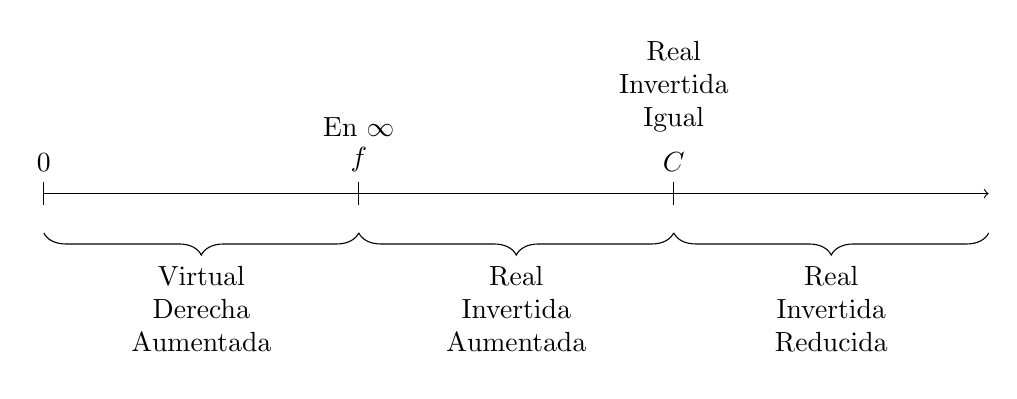
\begin{tikzpicture}

	% Línea principal
	\draw[->] (0,0) -- (12,0);

	% Marcas
	\draw (0,0.15) -- (0,-0.15);
	% \draw (4,0.15) -- (4,-0.15);
	\draw (4,0.15) -- (4,-0.15);
	\draw (8,0.15) -- (8,-0.15);
	% \draw (12,0.15) -- (12,-0.15);

	% Etiquetas arriba
	\node[above] at (0,0.15) {$0$};
	% \node[above] at (4,0.15) {$d_o$};
	\node[above] at (4,0.15) {$f$};
	\node[above] at (8,0.15) {$C$};

	% TEXTO ARRIBA de f
	\node[above] at (4,0.6)
	{
		En $\infty$
	};

	% TEXTO ARRIBA de C
	\node[above] at (8,0.6)
	{
		\begin{tabular}{c}
			Real      \\
			Invertida \\
			Igual
		\end{tabular}
	};

	% Llave izquierda
	\draw[
		decorate,
		decoration={brace,mirror,amplitude=8pt}
	]
	(0,-0.5) -- (4,-0.5);

	\node at (2,-1.5)
	{
		\begin{tabular}{c}
			Virtual \\
			Derecha \\
			Aumentada
		\end{tabular}
	};

	% Llave central
	\draw[
		decorate,
		decoration={brace,mirror,amplitude=8pt}
	]
	(4,-0.5) -- (8,-0.5);

	\node at (6,-1.5)
	{
		\begin{tabular}{c}
			Real      \\
			Invertida \\
			Aumentada
		\end{tabular}
	};

	% Llave derecha
	\draw[
		decorate,
		decoration={brace,mirror,amplitude=8pt}
	]
	(8,-0.5) -- (12,-0.5);

	\node at (10,-1.5)
	{
		\begin{tabular}{c}
			Real      \\
			Invertida \\
			Reducida
		\end{tabular}
	};

\end{tikzpicture}